% Chapter 1

\chapter{Introduction} % Main chapter title

\label{Chapter1} % For referencing the chapter elsewhere, use \ref{Chapter1} 

\lhead{Chapter 1. \emph{Introduction}} % This is for the header on each page - perhaps a shortened title

\setstretch{1}
%----------------------------------------------------------------------------------------
\section{About recommendation engine industry:}
 
 Recommendation engines aim at providing personalized suggestions to its users based on their behavior and taste, thereby reducing time taken to search a particular product or information in the web. Most of the recommendation engines are website based, few noticeable industry participants are Amazon, \acrshort{IMDB}, Flip-kart, eBay, Google, Linked-in, Facebook and Netflix. Main purpose of recommender websites is to cater for need of the customer by providing suggestive list of web pages as in case of Google, or to suggest relevant jobs as in the case of Linked-in or it could be suggesting next product to buy for users as in the case of on-line retail stores. Facebook uses it to filter posts from friends and for suggesting new friends, it is also used to predict movies matching to user's preference and tastes as in the case of Netflix. Recommendation engines have gained popularity with the advent of big data, a lot of startups have been created based on the idea of providing recommendations to its users. It helps users by filtering humongous amount of irrelevant data and by providing most relevant suggestions. Based on type of data used by recommendation engines, it is capable of either suggesting movies, restaurants, products or books to its users \citep{Recom0}. 

 Our main concern is about movie recommendation engine industry, which is built on data related to movies provided by movie industry from all over the world. Considerable amount of movies are added into movie database from movie producers each year, it is to be noted that there are more than hundred million movie titles in \acrshort{IMDB}, a largest on-line movie database \citep{IMDb2}. It also contains information about movie related data such as character, actor, popularity based information. Given this amount of data involved, movie data can be safely classified as big data. Currently there are about 15-20 companies in the area of on-line movie recommendations by either providing suggestions based on movie content, based on collected data from users or using both to predict and provide better suggestions. The top five companies in this domain are listed in decreasing order of popularity, they are \acrshort{IMDB}, Fandango, Rotten tomatoes, Flixster, What to rent ?. 

 A on-line movie on demand company, Netflix utilizes the power of movie recommendations to increase its customer engagement and it has also reported that due to recommendations, the subscriber growth is in the range of 10 to 30 percent \citep{Here1}. Movie recommendation engines are quite popular among movie enthusiasts, live example is popularity of \acrshort{IMDB} website with an average monthly traffic of 15 million users in USA alone \citep{Imdb8}, making it one of the top hundred most visited websites in the world as shown in \citep{Alexa5}. The example provided above establishes the fact that there is an imminent demand for movie recommendation engines and also in future due to monotonic increase in addition of new movies into the database. 

 It is clear from the above context that there is future for companies building movie recommendation engine. Competition is fierce due to involvement of major players in recommendation systems, namely \acrshort{IMDB}. There is a need for innovation in movie data analytics area and also in the domain of accurately predicting behavior of users to improve the state of movie recommendations provided. Availability of open source movie data reduces barriers for a new company to enter into recommender market. Typically, a company with a most innovative recommender algorithm involving in-depth movie content analysis, social data analytics, excellent user friendly framework for content discovery and moderate web infrastructure would be able to reach out to customers from all around the world with the help of a website. Generally, in the area of movie recommendation engines revenue models are based on advertisements in web space, royalties for publishing movie information, movie tickets sales, sales of collected customer data to other companies and end user subscription based revenue model.       

\section{About the company and its product:}
 Internship is carried out in a five year old startup company named Vion Labs, Stockholm. It is a digital media technology startup which focuses on providing a state of the art, innovative and appealing product for movie enthusiasts in the form of movie recommendation engine. A recent study by eMarketer in USA expects that an US adults to spend around 5 hours 46 minutes of their time per day in getting involved in digital media \citep{Mobil1}. As per movie on demand provider NetFlix, it has been observed that a average subscriber spends approximately 1 hour and 44 minutes streaming the video content \citep{HowM2}. From these studies it is clear that an average person spends most of his leisure time involving activities like watching movies, television and playing games in the digital world. Hence our startup has been focusing on digital media market to target a large number of customers in this segment. 

The method used for describing product or a service provided by a company is based on these following areas:
 
  \subsection{Features} % (fold)
  \label{sub:features}
  % subsection features (end) 
  The stand out and most attractive attributes that a company can offer in a product is a feature. The latest product of Vion labs is named as  ``Vionel'', which is a website with a personalized movie discovery platform. It has an appealing user friendly front end containing information about latest movies. It also has information about content providers, from where the users can get access to the video content. One of the attractive feature of Vionel is that it provides a social media type of platform to share personal views, likes and dislikes about a movie in the form of comments.
  
  The recommendation engine assigns a rating percentage score based on popularity of a movie, which helps user to chose movies with highest ratings. The front end of website provides user with the options to list movies based on different genres, keywords and characters involved. The feature of searching movies based on the tags for example,``adventure, action,comedy etc'' is also a part of Vionel's front-end.

  Vionel provides its users with a lot of different dimensions for critically analyzing movies. Future features to be included in website include relationship graphs among characters in the movies. Advertisement free web interface is one of the stand out feature of Vionel product, which creates a non-intrusive environment for the users to browse through movies. On the other hand it provides an excellent platform for the partner companies and other movie franchises to publish their movies in website.      
      
  \subsection{Advantages} % (fold)
  \label{sub:Advantages}
  % subsection subsection_name (end){Advantages} 
  Vionel is capable of providing its users with an state of the art movie content discovery platform unlike its competitors. The main advantage of Vionel is that it provides an user friendly social media platform for discussing and sharing one's view about the movies and the characters in the movies.

  The feature of bookmarking one's choice of movies and storing it in one's profile is a new feature in web movie database websites and Vionel has this feature. Vionel provides movie franchise owners to advertise their movies and trailer videos related to the movie. It also provides movie creators with social advertisement platform to collect opinions about movies from the viewers.      	   
   
  \subsection{Returns for the customer}
  \label{sub:Returns for the customer}

  Vionel provides its customers with a free website to enrich their movie selection experience. It provides users with a personalized movie discovery website with option to bookmark movies and also provides pointers to where the users can access the movie content. It also provides a user friendly social environment to discuss one's views about the movies. The website provides a one stop solution for all the movie enthusiasts to ponder upon latest content in the entertainment world and stumble upon movie to watch in lesser time than searching in web. It provides the movie creators and its advertisement agencies to showcase trailers of the movies. It enables movie franchises to collect valuable opinions and general public comments about the movies. Finally, the new and innovative features that are planned to be a part of Vionel product are from the internship work of automatic brand logo detection in movies to generate tag or category of movies namely ``Movies with product placement''. Along with recommendation engine this tag is used to provide better suggestions for the users of Vionel. Thereby assisting the movie recommendation engine to showcase the list of best possible movies based on user's choice and search behavior.      
 
%----------------------------------------------------------------------------------------
\section{Details about major thesis and its relevance}
% Explain about logo detection in movies, product placement in movies, how it can be automated way of creating a separate tag as an input to movie recommendation engines. Currently how rotten tomatoes, \acrshort{IMDB} are creating this tag ? {using user's reviews and comments}. This process can be automated and credibility of the data can be maintained. Block diagram of the movie recommender engine (Write this in essay part of the report ) Which Phase ? Why so ? %
%----------------------------------------------------------------------------------------
 Goal of major thesis and internship is to develop a automatic brand logo detection in input movies. Recognition, identification of brand logos in movies is a arduous and error prone task to be carried out by humans. In order to accelerate the process of detecting logos and also to increase the accuracy of detection in movies a machine learning algorithm combined with computer vision algorithms are used. The process of analyzing more than hundred million movies to detect the presence of brand logos is a time consuming process, hence in the project a cluster of state of the art graphical processing units are used to accelerate the process. After detection of logos, movies are tagged as containing product placement in them. The tags generated for all the movies are collected and used as input to movie recommender system. An instance of the use case is, when a user has liked watching movie with product placements, it is highly likely a user may like another movie with similar tag. Hence in order to increase the reliability of movie recommendation engine, a lot of such features has to be developed. The deliverable of internship will be to automate the process of movie logo detection and generate output in a predefined structure, to be later used by recommender system. Currently brand logo detector is in prototyping phase of software development cycle.

\section{Current phase in innovation process} 
%----------------------------------------------------------------------------------------
 % About the process and current phase of minor thesis 
 Company has developed a \acrshort{MVP} in the form of a movie information publishing and discovery platform. The \acrshort{MVP} has been launched in the market as a website named \href{www.vionel.com}{Vionel}. The baseline release of the product has the feature of allowing users to search for movie information, provide comments about movie content, share and bookmark movies. It lacks recommendation engine that provides user with personalized recommendations based on data collected from behavior of users. Hence current goal of research and development team of the company is to develop a state of the art movie recommender engine, which provides a reliable set of movie recommendations to the end user. 
 \par Since recommendation engine is a new feature going to be added on top of baseline product, there is need to study business aspects like demand from customers, current market scenario and about competitors. Recommendation engine product is currently in ideation phase of innovation process framework. In this phase R\&D team brainstorms about type of recommender system to use, set of innovative features to be included and aspects about increasing accuracy of suggestions. One such feature is part of my internship project involving automatic brand logo detection in movies, which is currently in prototyping phase of its software development cycle. The final output of master thesis project is to produce tag information for movies with product placements, it will be one of the many inputs for final recommender engine product. Likewise, there are other innovative features that could be included as part of the movie recommendation engines, such as creation of tags for movies with a particular type of environment (ex: Indoor, Forest, Urban etc). 
 \par Prior to ideation phase in innovation process, two important steps has to be performed. First one is to investigate needs and demands of the customer in recommender system context. Second step is to investigate about current market situation for product that is intended to be created. These two steps clears out the confusion regarding acceptance of end product by customers. The next step is to understand competition in the field by performing competitor analysis. Subsection \ref{Voice} explains about problems, needs and demand of customer in recommender engine context and it also gives insight about current market scenario in web based recommender systems.

 \subsection{Voice of the customer}
 \label {Voice}
  % Movie recommendations acceptance poll by the customers (a graph may be). Need for recommendations, what problems are faced by the customer currently ? How our solution mitigates it ? Demand discovery. Block diagram of voice of customer, explain each of the blocks. 
  Customer demand always drives success of a product. Discovery, timely identification and capitalization of customer demand about a particular product is essential for development of a company. Value proposition as perceived by customer should be in positive note, also a product or service should be a able to solve a problem faced by the customer. During initial phase of market study, needs, expectations and preferences of movie recommendation engines are studied.
  \par
  In the case of simple movie discovery and information retrieval websites, customers face problem of manually searching movies they want to watch at that instant and it is a time consuming task especially if the number of choices are large in number. This is a problem, since each time a user logs into a movie discovery website, the set of movies displayed will be static with latest movies getting priority of moving up the list. The list presented is identical for all the users, which makes majority of users to leave the service. Hence it is observed that customers need a personalized list of movie suggestions based on their taste, mood, time and day of the week and other user information. It is also noticed that when an average user has no preference about movie to watch, always takes suggestions from a friend before watching a movie. This limits the possibilities of movies suggested by a friend, this demands recommendation engines to be automated and personalized to enrich and surprise users by providing diversified set of movie suggestions when compared to suggestion from a friend.
  \par 
  Direct demands and other implicit information about a product is obtained using a market survey. One such survey conducted in 2010 as in figure \ref{fig: Familiarity of recommendation engines} showed that more than 80 percent of the respondent population either showed interest in recommendation engines or currently using one \citep{Recom8_voc}. This study reveals information about the familiarity of recommendation engines by customers. 
 
  \begin{figure}[htbp]
	\centering
		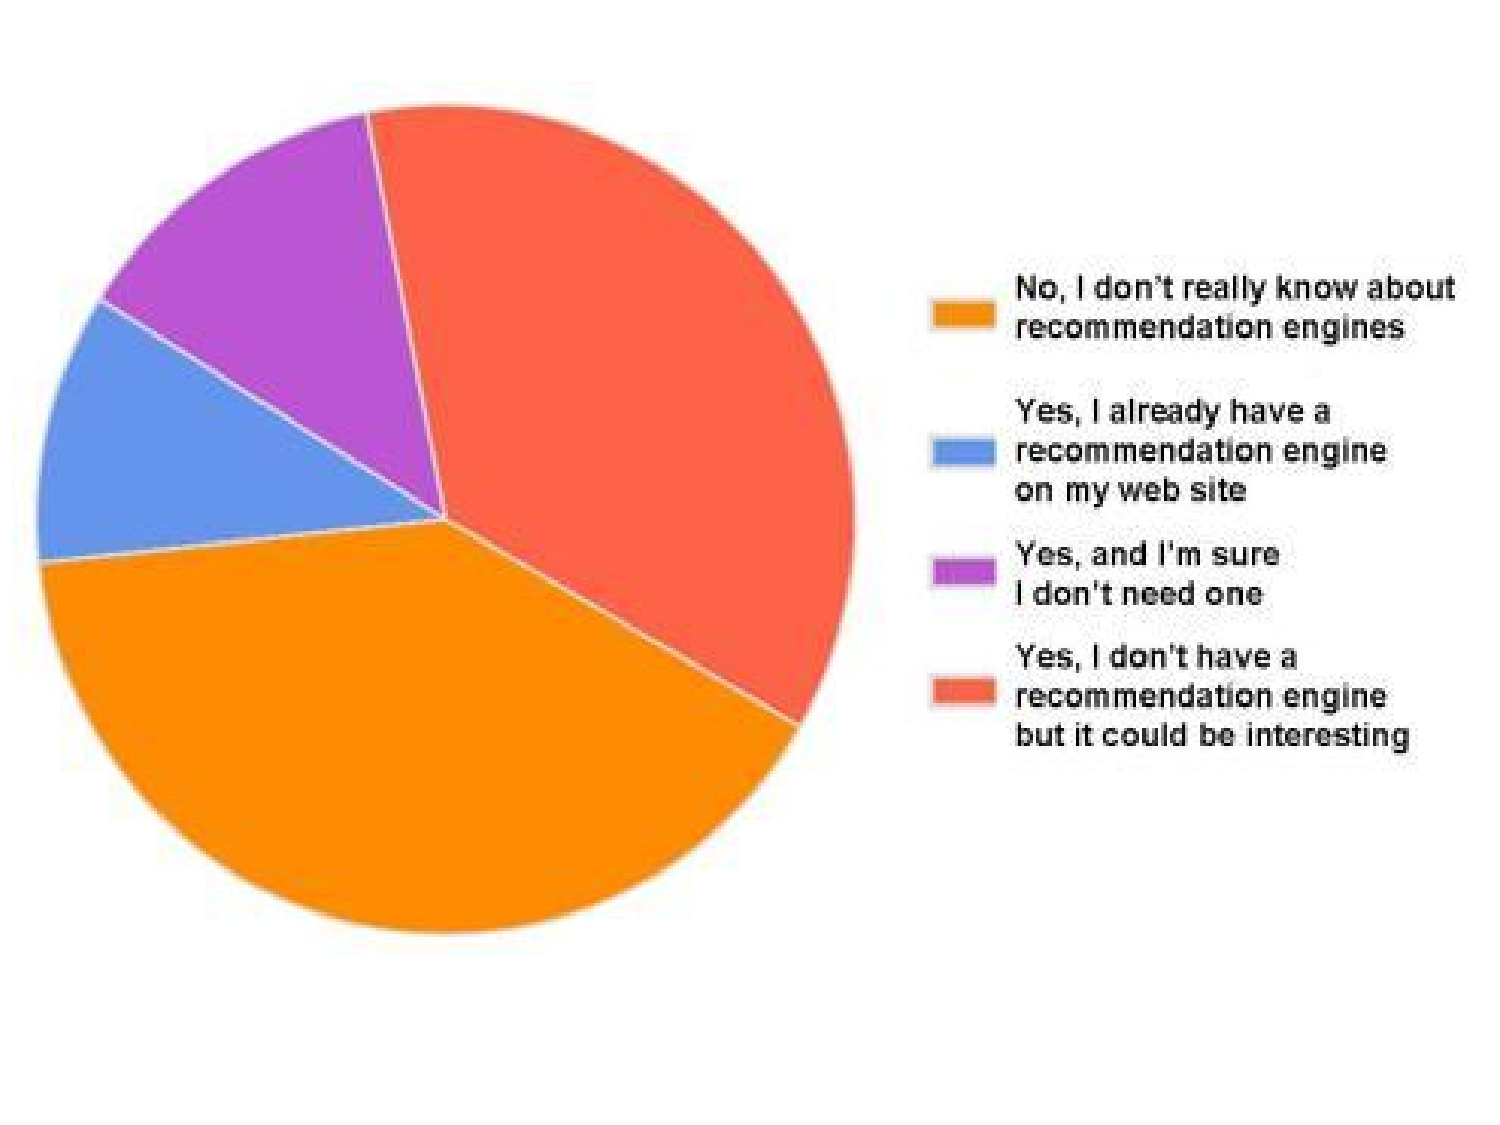
\includegraphics[scale=0.4]{Figures/familiarity_recommendation_engines.pdf}
		%\rule{35em}{0.5pt}
	\caption[Graph: Familiarity of web based recommendation systems]{A survey results on familiarity of recommendation engines \citep{Recom8_voc}.}
	\label{fig: Familiarity of recommendation engines}
  \end{figure} 

  Public relation(PR) team members in Vion Labs have been able to build a good relationship with current users of Vionel using social media and emails. Customer view about the product is obtained from feedback forms in the website. Evenmore personalized review comments about website and its content are obtained by sending out emails for first five hundred privileged users. Complaints, suggestions about movie information are logged and periodically checked to improve the service. The availability of baseline website made the process of understanding customer views about inclusion of recommender system using surveys a easy task, the response gathered is positive about movie recommendations inclusion. Vionel is a free website for users from all over the world, along with that inclusion of state of the movie recommendation enriches movie selection experience of customers. In order to gain even more insights from customers, an interactive video linked with a on-line survey was prepared and published to gather information. In conclusion, there is a positive demand for movie recommendation engine by end users. 

  Marketing team have gathered information about benefits for partner companies and movie franchises, by inclusion of recommendation features on top of baseline product. It has been observed that movie recommendations diversifies the spread of movies chosen by users and thereby increasing the sales of less familiar DVDs and video content from partner websites such as Netflix. This boosts movie content that is not so popular among public, hence movie on demand services can benefit from less familiar movies available in unprofitable part of long tail distribution of movies as discussed in \citep{Profile_online}.

  Even though, initial analysis of customer needs, problems and expectations are accomplished, there is a room to investigate more and understand average customer expectations about movie recommendation engines. The view of recommendations as perceived by the user, will highly influence both technical and business decisions during the development of \acrshort{MRS}. More customer insights about outlook of a recommender system is to be collected using customer interviews, surveys and discussion with movie franchise owners. More data needs to be collected about user's opinion on intrusion levels of privacy for collecting user behavioral data on website such as clicking pattern on displayed movie information, movie posters viewed, searching pattern for movies, comments, bookmarks, likes and dislikes of displayed movies.

  Marketing team in Vionel have collected information from web regarding market share information of recommendation engines. Google page rank of websites provide information about the number of unique views of the website, which is used to calculate market share of various recommendation engines. Sector graph in figure shows the market share information of the websites the data is collected and computed from from \citep{Alexa_imdb}. It is assumed that the company which has least rank has highest market share. It is observed that \acrshort{IMDB} has captured a market share of more than 88 percent. The reason is due to it sheer movie information database and presence of user ratings. There is still room for conducting market survey to understand about competitors in current scenario.      
   
  \begin{figure}[htbp]
	\centering
		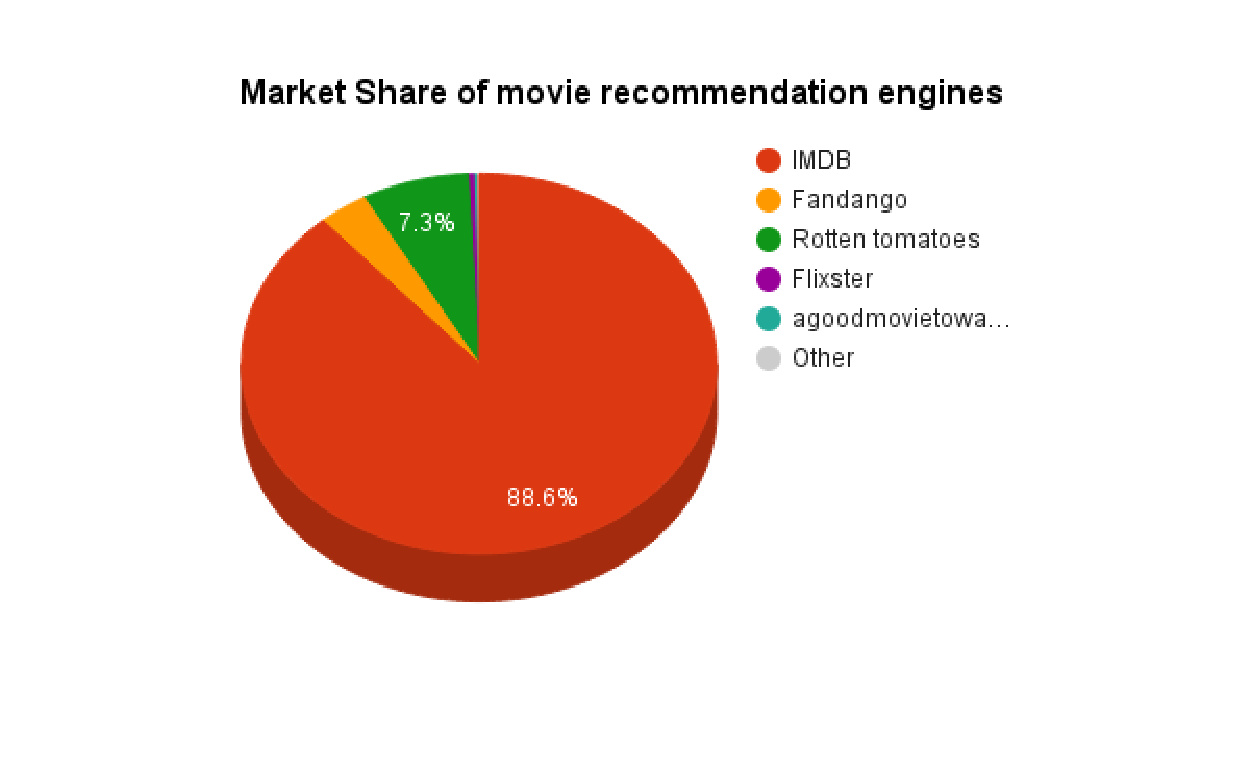
\includegraphics[scale=0.5]{Figures/Market_share.pdf}
		%\rule{35em}{0.5pt}
	\caption[Sector graph: Market share of web based recommendation systems]{Market share of web based movie recommendation engines \citep{Alexa_imdb}.}
	\label{fig: Market share information of web based movie recommendation systems}
  \end{figure} 

% \subsection{Market analysis}
% \label {Market}

 % What is it ? its importance ? its role in driving innovation strategy ? 
 
 % Real market facts and figures, market share, TAM,
 
 % Ideation of the product : Unique features inclusion into baseline product.
 

\section{Framing of business research question in the given context}
%----------------------------------------------------------------------------------------
 % How to achieve competitive edge, comparison of tech, business features, marketing strategies, strategic alliances made by other companies, attaining competitive sustainable advantage---> The process (innovative framework) for quick reference comparison.  
 Baseline version of the product Vionel has been launched in the market, but it lacks movie recommendation engine. There has been a considerable amount of effort spent in understanding needs, problems and expectations of customer regarding movie recommendation engines. The second part of the study involved study of market in context to acceptance of movie recommendation engines. A movie recommendation engines is an ensemble of various features both related to movie content and user behavior. Development and inclusion of each feature for a movie recommendation engines is a project with an aim of analyzing movies and generating movie tags in an innovative way. The reliability, accuracy and popularity of \acrshort{MRS} depends on the features it has and quality of tags it holds. 

 As a step along innovation process framework it is required to understand about competitors in movie recommendation engines, features used and provided to the end users. Comparison with competition helps us to improve the present condition of \acrshort{MRS} by either addition or deletion of features. Knowing about competition much before ideation phase of innovation process, helps R\&D team members to collaborate and come up with quality features to be added on top of baseline version. So there is a benefit of performing detailed analysis about competition to further reduce the development time of \acrshort{MRS}. This helps company to achieve shorter time to market for the product by taking appropriate measures during ideation phase of the product. Hence the research question that will be answered in this minor thesis would be about  

 \textbf{RQ}: \textbf{``How to investigate with a creative approach and compare features provided by movie recommendation engine firms. Also based on this, to develop a consistent understanding of how technological differentiation in technical features of a movie recommender website would attract more number of users to gain sustainable competitive advantage in an innovative way ?''}